\documentclass{article}
\usepackage{tikz-cd}
\usetikzlibrary{calc}

\begin{document}

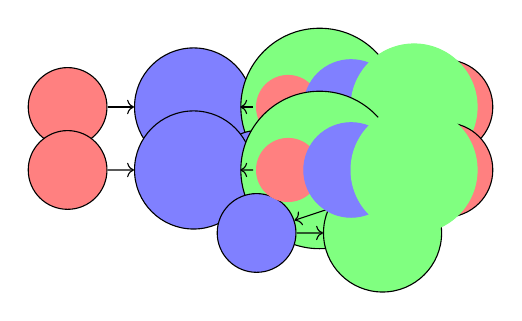
\begin{tikzpicture}[scale=0.8]
    \node (A) at (0,0) [circle, draw, fill=red!50, minimum size=1cm] {};
    \node (B) at (2,0) [circle, draw, fill=blue!50, minimum size=1.5cm] {};
    \node (C) at (4,0) [circle, draw, fill=green!50, minimum size=2cm] {};
    \node (D) at (6,0) [circle, draw, fill=red!50, minimum size=1.2cm] {};
    \node (E) at (3,-1) [circle, draw, fill=blue!50, minimum size=1cm] {};
    \node (F) at (5,-1) [circle, draw, fill=green!50, minimum size=1.5cm] {};
    
    % Draw arrows for the TikZ-CD
    \draw[->] (A) to node {} (B);
    \draw[->] (B) to node {} (C);
    \draw[->] (C) to node {} (D);
    \draw[->] (D) to node {} (E);
    \draw[->] (E) to node {} (F);
    
    % Overlapping circles
    \filldraw[red!50] (3.5,0) circle (0.5cm);
    \filldraw[blue!50] (4.5,0) circle (0.75cm);
    \filldraw[green!50] (5.5,0) circle (1cm);
    
    % Adjusting the positions of the nodes to avoid overlap
    \node (A') at (0,-1) [circle, draw, fill=red!50, minimum size=1cm] {};
    \node (B') at (2,-1) [circle, draw, fill=blue!50, minimum size=1.5cm] {};
    \node (C') at (4,-1) [circle, draw, fill=green!50, minimum size=2cm] {};
    \node (D') at (6,-1) [circle, draw, fill=red!50, minimum size=1.2cm] {};
    \node (E') at (3,-2) [circle, draw, fill=blue!50, minimum size=1cm] {};
    \node (F') at (5,-2) [circle, draw, fill=green!50, minimum size=1.5cm] {};
    
    % Draw arrows for the TikZ-CD
    \draw[->] (A') to node {} (B');
    \draw[->] (B') to node {} (C');
    \draw[->] (C') to node {} (D');
    \draw[->] (D') to node {} (E');
    \draw[->] (E') to node {} (F');
    
    % Overlapping circles
    \filldraw[red!50] (3.5,-1) circle (0.5cm);
    \filldraw[blue!50] (4.5,-1) circle (0.75cm);
    \filldraw[green!50] (5.5,-1) circle (1cm);
\end{tikzpicture}

\end{document}